\documentclass{report}

% Language setting
% Replace `english' with e.g. `spanish' to change the document language
\usepackage[english]{babel}

% Set page size and margins
% Replace `letterpaper' with `a4paper' for UK/EU standard size
\usepackage[letterpaper,top=2cm,bottom=2cm,left=3cm,right=3cm,marginparwidth=1.75cm]{geometry}

% Useful packages
\usepackage{amsmath}
\usepackage{graphicx}
\usepackage{float}
\usepackage{subcaption}
\usepackage[colorlinks=true, allcolors=blue]{hyperref}

\newtheorem{definition}{Definition}[section]

\title{Protein Structures}
\author{Vinay Kakkar}

\begin{document}
\maketitle

\tableofcontents

\begin{abstract}

Three-dimensional structure are created from sequences of amino acids in polypeptide chains folds that generate from linear chains. The folded domains can serve as modules for building up large assemblies such as a muscle fiber but more importantly, they can provide specific catalytic or binding sites, as found in enzymes or proteins. We look at the fondations of a protein such as the building blocks. Using technologies in order to read these sequences of amino acids into information that helps determine what the function of the structre will have. Using our knowladge of protien structres and Bioinformatics we can achive the goal of predicting functions of proteins from a large set of data provided by experiments such as, DNA microarray technology and Two-dimensional Gel electrophoresis or Chromatography. With new technologies such as AlphaFold we can even predict the 3D structure of a Protein using the amino acid sequence alone.

\end{abstract}

\renewcommand\thesection{\arabic{section}}

\section{Introduction}
Amino acids are molecules that combine to form proteins. All of the 20 amino acids see table~\ref{Amino acids} have in common a central carbon atom which are attached a hydrogen atom, an amino group and a carboxyl group. What distinguishes one amino acid from
another is the side chain attached to the central carbon atom through its fourth valence~\cite{branden_introduction_1998}.

\begin{table}[h!]
    \begin{center}
    \label{tab:Amino acids}
        \begin{tabular}{l|c|r}
        Amino acid & Three-letter code & One-letter code\\
        \hline
        \\
        Glycine & Gly & G\\
        Alanine & Ala & A\\
        Valine & Val & V\\
        Leucine & Leu & L\\
        Isoleucine & Ile & I\\
        Proline & Pro & P\\
        Phenylalanine & Phe & F\\
        Methionine & Met & M\\
        Tryptophan & Trp & W\\
        Cysteine & Cys & C\\
        \\
        \hline
        \\
        Asparagine & Asn & N\\
        Glutamine & Gln & Q\\
        Serine & Ser & S\\
        Threonine & Thr & T\\
        Tyrosine & Tyr & Y\\
        \\
        \hline
        \\
        Aspartic acid & Asp & D\\
        Glutamic acid & Glu & E\\
        \\
        \hline
        \\
        Histidine & His & H\\
        Lysine & Lys & K\\
        Arginine & Arg & R\\
        \end{tabular}
        \caption{\label{Amino acids}The 20 amino acids. The amino acid name, the three-letter code, and the one-letter code are given. The Amino acids are split up into Nonpolar, Polar, Acidic and Basic respectfully}
    \end{center}
\end{table}

Proteins are responsible of catalysing almost all the chemical reactions in the cell. Proteins can function as enzymes catalysing a wide variety of reactions vital for life thus being important for the structure of living systems such as those proteins involved in the cytoskeleton. The size of protein can vary from small to quite large macromolecules~\cite{zvelebil_understanding_2008}.

\begin{definition}[Catalysing]
    Catalysing is to make a chemical reaction happen or happen more quickly by acting as a catalyst.
\end{definition}

\begin{definition}[Cytoskeleton]
    A dynamic network of interlinking protein filaments present in the cytoplasm of all cells~\cite{zvelebil_understanding_2008}. 
\end{definition}

Given that protiens are a built up off of amino acids, we can analyse a DNA sequence of a gene to retrieve the amino acid sequence of the protein product. Using this and Bioinformatics we can help deduce the likely properties of unknown proteins, whilst including their functions and structures. Knowing the relationship between a proteins structure and its function provides a greater understanding of how the protein works and thus enables experiments to explore how modifying the structure will affect the function. Interacting with proteins, structure-function studies are vital to the design of new drugs, the use of bioinformatics exelerates this process aswell as providing computer modelling of these interactions~\cite{zvelebil_understanding_2008}.

\section{Protein Structure}

\subsection{Primary, Secondary, Tertiary and Quaternary Structure}

\subsubsection{Primary Structure}

The primary structure of a peptide or protein is the linear sequence of its amino acids (AAs). The primary structure of a protein is read and written from the amino-terminal (N) to the carboxyl-terminal (C) end. Each amino acid is connected to the next by a peptide bond~\cite{noauthor_levels_nodate}.

\subsubsection{Secondary Structure}

Compared to the primary structure which describes the sequence of amino acids forming a peptide chain, secondary structure refers to the local arrangement of that chain. Where several common secondary structures have been identified in proteins~\cite{noauthor_levels_nodate}.

\subsubsection{Tertiary Structure}

Tertiary structure is a three-dimensional structure of a protein which when compared to the primary strucutre sequence it can interact with one another to form secondary structures such as helices and sheets, and individual amino acids from distant parts of the primary strucutre sequence can intermingle. The formation of these bonds and interactions serve to change the shape of the overall protein. The folding that we end up with for a given polypeptide is the tertiary structureZ\cite{godbey_chapter_2022}.

\subsubsection{Quaternary Structure}

Quaternary structure of a protein is the association of several protein chains or subunits which are closely packed arrangement. Each of the subunits has its own primary, secondary, and tertiary structure. The subunits are held together by hydrogen bonds and van der Waals forces between nonpolar side chains~\cite{ouellette_14_2015}.

\begin{definition}[Van Der Waals]
    A relatively weak electric force that attract neutral molecules that collide with or pass very close to each other~\cite{noauthor_210_2018}.
\end{definition}

\begin{center}
    \begin{tabular}{l|c|r}

    \end{tabular}
\end{center}

\begin{table}[h!]
    \begin{center}
    \label{tab:Quanternanry Protiens}
        \begin{tabular}{l|c|r}
            \hline
            Protein & Number of Subunits & Function\\
            \hline
            Alcohol dehydrogenase & 4 & Enzymatic reaction in fermentation\\ 
            \hline
            Aldolase & 4 & Enzymatic reaction in glycolysis\\
            \hline
            Fumarase & 4 & Enzymatic reaction in citric acid cycle \\
            \hline
            Hemoglobin & 14 & Oxygen transport in blood\\
            \hline
            Insulin & 2 & 6344\\
            \hline
        \end{tabular}
        \caption{\label{Quanternanry Protiens}Examples of Proteins Having Quaternary Structure~\cite{ouellette_14_2015}.}
    \end{center}
\end{table}


\begin{figure}[H]
    \centering
    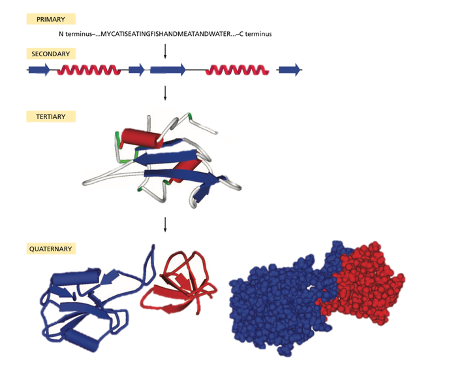
\includegraphics[width=0.5\textwidth]{Protein Structure.png}
    \caption{\label{fig:Simple schematic showing the different levels of protein structure.}From the sequence alone (the primary structure) to secondary structure (which contains local structural elements), to tertiary structure (where the structural elements fold to give a three-dimensional structure), to finally quaternary structure found when several tertiary structures form a multisubunit complex~\cite{zvelebil_understanding_2008}.}
\end{figure}

\subsubsection{Considering Protein structure on several different levels}

Protien folds into a three-dimensional tertiary structure from repeating secondary structures, which is determined by its protein sequence. The fold of the protein is important for the way the protein will function, and whether it will function correctly. Therefore the study of the ways in which proteins fold with understanding how they fold is an important area of bioinformatics~\cite{zvelebil_understanding_2008}. For example predicting the fold of a protein from its sequence. We can then go further and use computational analysis on these predictions.

When considering Protein structures on different levels we can look into; The analysis of protein structure by experimental techniques such as X-ray crystallography and nuclear magnetic resonance (NMR) which show that proteins adopt distinct structural elements~\cite{zvelebil_understanding_2008}. 

The structure adopted by a protein chain, and thus its function, is determined entirely by its amino acid sequence, but the rules that govern how a protein chain of a given sequence folds up are not yet understood and it is impossible to predict the folded structure of a protein de novo from its amino acid sequence alone Helping to solve this problem is one of the challenges facing bioinformatics~\cite{zvelebil_understanding_2008}.

\begin{definition}[De novo]
    The first occurrence of cancer in the body.
\end{definition}

\subsubsection{Amino Acids}

Amino acids are covalently linked together in the protein chain by peptide bonds. The primary structure of a protein is the sequence of amino acids in the linear protein chain, which consists of covalently linked amino acids. This linear chain is often called a polypeptide chain~\cite{zvelebil_understanding_2008}.

Amino acids are different to each other due to their side chains. The functional properties of proteins are almost entirely due to the side chains of the amino acids. Each type of amino acid has specific chemical physical properties that are conferred on it by the structure and chemical properties of its side chain. They can, however, be classified into overlapping groups that share some common physical and chemical properties, such as size and electrical charge. Some side chains can be charged and not charged they can even be negatively or positively charged~\cite{zvelebil_understanding_2008}.


\begin{figure}[H]
    \centering
    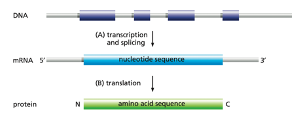
\includegraphics[width=0.5\textwidth]{Transcription and translation.png}
    \caption{\label{fig:Transcription and translation}The relation of DNA coding-strand sequence to mRNA sequence to protein sequence. The exons (purple boxes) of the DNA are transcribed into mRNA which, using other molecules directs the protein sequence~\cite{zvelebil_understanding_2008}.}
\end{figure}

\subsubsection{Bioinformatic Difficulties with Predictions on Proteins}

Secondary structure of proteins is made up of a-helices and b-strands. It should be noted that the structures found in globular proteins are not perfectly regular, so it is frequently difficult to define the precise ends of the helices, and in some cases the hydrogen-bonding patterns are intermediate between these idealized forms. Therefore, prediction of these structures using bioinformatics programs is made more difficult~\cite{zvelebil_understanding_2008}.

Several different types of b-sheet are found in protein structures. Turns, hairpins, and loops connect helices and strands. Any chain between two regular structures is referred to as a loop. In many cases a loop will contain a turn (or even several). In general there are no classifications for loops, but there is an important exception. In antibody recognition, immunoglobulins employ loops at the edge of a b-sheet to recognize the antigen. There are vast numbers of different immunoglobulin structures, all with the same overall chain fold, but it is the difference at these loops that results in different affinities. With many structures known, it has been observed that the loops take up one of a limited number of structures (called canonical forms), so that in this particular case the loops have been classified. This type of classification is important when trying to predict both the structure and function of the protein~\cite{zvelebil_understanding_2008}.

\begin{definition}[Immunoglobulin]
    Immunoglobulins are heterodimeric proteins composed of two heavy (H) and two light (L) chains. Types of white blood cells that helps the body fight infection~\cite{schroeder_structure_2010}.
\end{definition}

\subsection{Compact Structures}

\subsubsection{Protein Folds}
Sole protein chains have little to none biological function. Only when the chain has folded up into a tertiary or quaternary structure it then has some functional activity ~\cite{zvelebil_understanding_2008}. For example:

Proteins enzymes bind to other molecules (ligands) and catalyze their biochemical reactions, we can have others that act by binding other proteins and influencing their activity, and yet others bind to DNA and regulate gene expression~\cite{zvelebil_understanding_2008}.

Other proteins have a purely structural function, making up the fabric of the cell. Large numbers of proteins acting as chemical messengers are released, from cells, influencing the behavior of other cells by acting on yet another large functional class of proteins, known as receptors, on cell surfaces~\cite{zvelebil_understanding_2008}.

The tertiary structure of a protein is defined by the path of the polypeptide chain In the tertiary structure of a protein, various combinations of secondary structure pack together to form a compactly folded mass. In a multidomain protein it is thought that each domain folds independently of the others~\cite{zvelebil_understanding_2008}.

\subsubsection{Bioinformatics with Protein Folds}

Bioinformatics questions are often concerned with comparing the sequences and structures of different domains rather than whole proteins. A domain can be anything from 50 to around 350 amino acids in length. The three dimensional structure of a protein is known as its conformation. More specifically, the spatial path of any given folded polypeptide chain is known as its fold~\cite{zvelebil_understanding_2008}.

There appears to be a limited number of ways in which secondary structures fold into domains. There are several instances where proteins that seem to be completely unrelated in terms of sequence are found to have the same fold and some researchers estimate that there may be only a few thousand different folds in nature. Currently, there are more than 35,000 known protein structures, and these are classified into approximately 2000 fold families. The fact that so many proteins fold into a similar structure even if their sequences are not very similar means that we can use bioinformatics tools to model structures of various proteins on similar folds~\cite{zvelebil_understanding_2008}.

\section{Large Scale Experssion}

Gene expression begins when genes are transcribed into messenger RNAs (mRNAs), which are then translated to produce proteins. Total gene expression in cultured cells or a tissue sample can be detected in two main ways:

\begin{enumerate}
    \item DNA microarray technology.
    \item Two-dimensional Gel electrophoresis or Chromatography.
\end{enumerate}

Both cases produce enormous amounts of raw data, thus new techniques had to be devised for data collection, storage, and analysis. The transcriptome and proteome, unlike the genome, are changeable in response to conditions, and depend on the state of development, the environment, and the type of tissue~\cite{zvelebil_understanding_2008}.

Monitoring the simultaneous expression of multiple genes provides information which can not be obtained by monitoring the expression of one gene. Looking at genes that are expressed together, or co-expressed, we can use technologies that can identify genes that may be functionally related. This can be used to help assign possible functions to unidentified genes with the same expression patterns. Co-expression can also help indicate which genes are under the control of the same regulatory system~\cite{zvelebil_understanding_2008}.


\subsection{Large Scale Gene Expression}

Genome DNA microarrays aid in biological research however, the interpretation of the large amount of data produced by a microarray experiment can be computationaly heavy on top different methods can yield alternative conclusions inceasing the computational effort. The goal of these experiments is to extract some biological or functional meaning from the lists of genes, either by:

\begin{enumerate}
    \item Identify critical genes that are responsible for a biological effect.
    \item Find patterns within the genes that point to an underlying biological process.
\end{enumerate}
\cite{zvelebil_understanding_2008}

\begin{figure}[H]
    \centering
    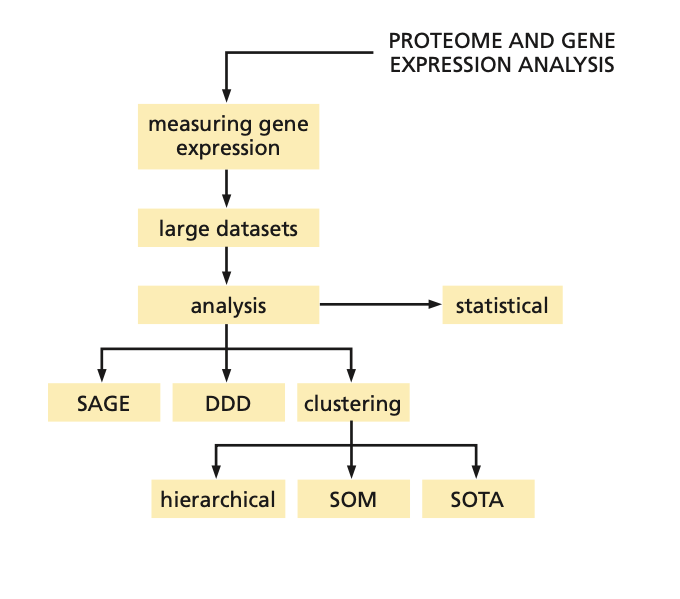
\includegraphics[width=0.5\textwidth]{Gene Expresion.png}
    \caption{\label{fig:Gene Expression}In this section common experimental aspects of gene expression and of the analysis of the resulting data are described~\cite{zvelebil_understanding_2008}.}
\end{figure}

\subsubsection{Serial analysis of gene expression}

Serial analysis of gene expression (SAGE) is alternative compared to microarrays for investigating patterns of gene expression.
We wil look into both the experimental and a bioinformatics component.

\begin{figure}[!h]
    \centering
    \begin{subfigure}[t]{.45\textwidth}
        \centering
        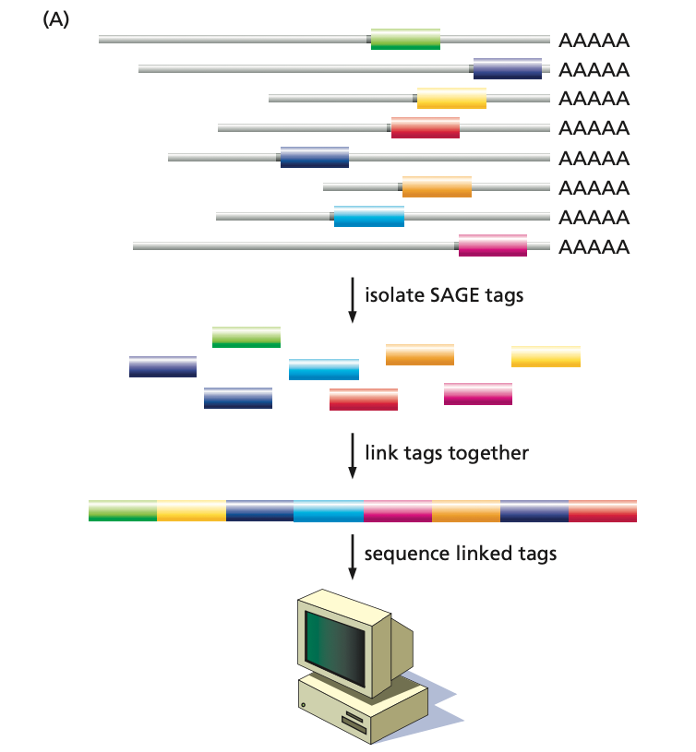
\includegraphics[width=0.9\textwidth]{SAGE1.png}
        \caption{}
        \label{fig:SAGE1} 
    \end{subfigure}
    \begin{subfigure}[t]{.45\textwidth}
       \centering
       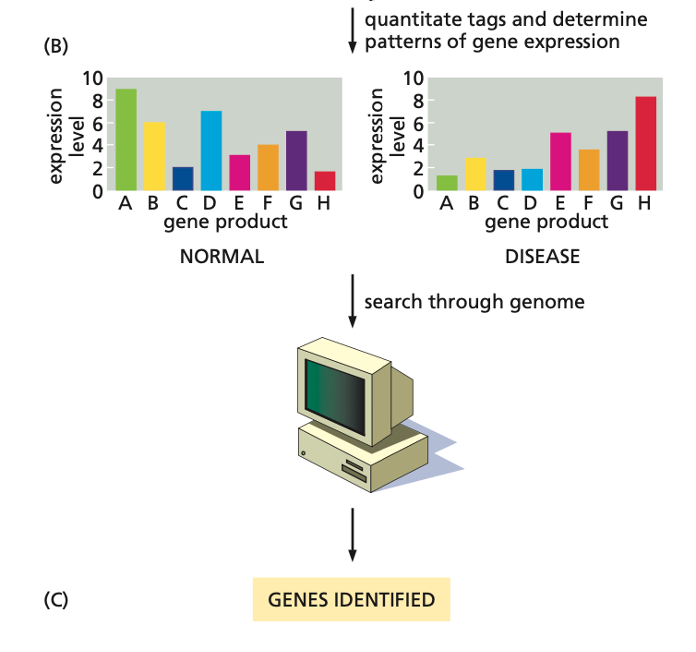
\includegraphics[width=0.9\textwidth]{SAGE2.png}
       \caption{}
       \label{fig:SAGE2}
    \end{subfigure}
    \caption{\emph{An outline of the SAGE method for comparing levels of gene expression. (A) Short sequence tags. The sequence tags are isolated and are linked together to produce long DNA molecules that can be cloned and sequenced. (B) Once sequenced, each tag can be calculated, resulting in a value that gives the expression level of the corresponding transcript~\cite{zvelebil_understanding_2008}.}}
    \label{fig:SAGE}
\end{figure}


First, that a short sequence (a tag) contains enough information to uniquely identify a gene. Then the sequence tags from the total cellular RNA can be linked together to form long DNA molecules. The total number of times a particular tag is observed in the concatemers approximates the expression level of the corresponding gene. The data produced by SAGE include a list of the tags with their corresponding counts, providing a digital output of cellular gene expression that can easily be analyzed further. Which allow the user to specify which organ is to be investigated. Libraries consisting of gene lists organized by the various types of tissues or cell lines are provided for further choice. The output from SAGE provides the SAGE tag, the UniGene ID, the gene description, and color and letter coded differences in expression levels~\cite{zvelebil_understanding_2008}.

\subsubsection{Detect differential gene expression}

Digital differential display (DDD) is a method for comparing EST-based expression profiles in different tissues or conditions from various libraries or between pools of EST libraries. An EST library contains short sequences cloned from the total cellular mRNA of a particular tissue or particular condition. The theory is that genes expressed at a high level will be represented by more ESTs than those expressed at a lower level. Genes whose expression levels differ significantly from one set of EST libraries to the next are identified using a statistical test~\cite{zvelebil_understanding_2008}.

In UniGene, all the human EST sequences in the databases have been put into distinct clusters, where each cluster represents a single gene. We then use a method to compare the number of sequences from each EST library assigned to a particular UniGene cluster, and identifies those differences between the clusters that are likely to be biologically significant~\cite{zvelebil_understanding_2008}.

\subsubsection{Clustered gene expression data}

Clustered data on gene expression patterns obtained from either gene expression microarrays or genome bioinformatics can be used as a predictive tool to identify new transcription factors or other cell-regulatory proteins. The clustered genes (or proteins) can be analyzed. This leads to a vast collection of data from many gene expression and protein expression expeniments being available on the Web to be used as reference data for the development of new bioinformatics tools~\cite{zvelebil_understanding_2008}.

\subsection{Large Scale Protein Expression}

\begin{figure}[H]
    \centering
    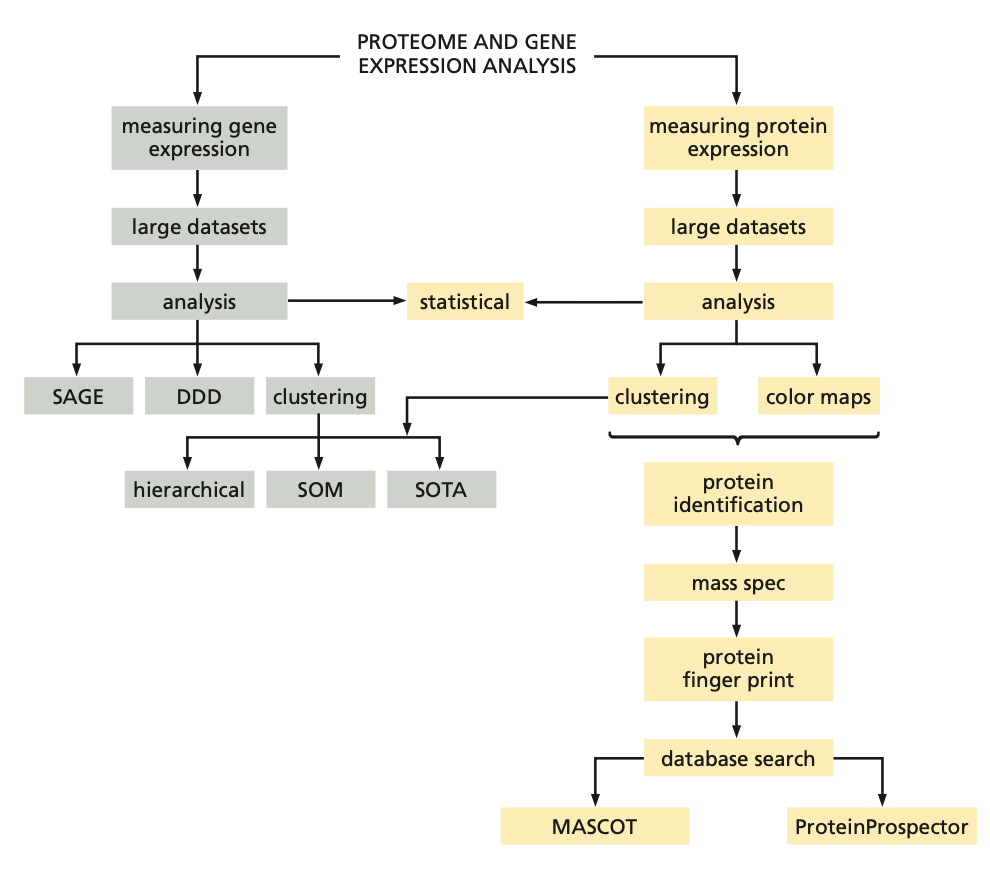
\includegraphics[width=0.5\textwidth]{Overlaping.png}
    \caption{\label{fig:Overlaping}This section describes some experimental aspects of protein expression and of the analysis of the resulting data, showing the overlap between gene and protein expression~\cite{zvelebil_understanding_2008}.}
\end{figure}

Measuring mRNA, however, does give us all we need to know for a gene expression. To obtain a functional protein, mRNAs have to be translated, and the protein products often undergo modifications that influence their function. For this reason we can measure and anlayse different proteins. There are many more proteins than there are genes in a genome, whilst many transcripts can be spliced in various ways to give different mRNAs, which in return provide different protein products, from the same gene, and proteins can be modified after translation giving more different protien products.

The proteome refers to all the proteins that make up an organism at a specific point in time and under specific conditions. As protien expressions can vary in a organism depending on the part it will also differ between the separate stages of an organism’s life cycle and under different environmental conditions. To understand how an organism or a cell functions both under normal and abnormal (such as disease) conditions it is important to know how protein expression is affected~\cite{zvelebil_understanding_2008}.

\subsubsection{Clustering methods to identify protein spots with similar expression patterns}

Clustering is a useful method of extracting protein expression patterns that can indicate biological differences or similarities between samples. Many of the clustering methods used for microarray data can be applied to 2D gel data.~\cite{zvelebil_understanding_2008}.

\section{Alpha Fold}

The AlphaFold network directly predicts the 3D coordinates of all heavy atoms for a given protein using the primary amino acid sequence and aligned sequences of homologues as inputs~\cite{jumper_highly_2021}.

AlphaFold is a major advancement with the aim to predict a protein’s structure from its amino acid sequence alone. In nature, proteins reliably fold into precise 3D conformations that is critical for its function based on nothing more than the sequence of amino acids that it is composed of\cite{felix_brief_nodate}

In fact, mutations in proteins that lead to misfolding are often associated with disease states, for example, Alzheimer’s and Parkinson’s~\cite{felix_brief_nodate}.

The final output of AlphaFold is a file containing the 3D coordinates for every non-hydrogen atom in the protein. It also outputs a graph showing the confidence levels for every amino acid residue, which allows users to assess the reliability of the predicted structure~\cite{felix_brief_nodate}.

\subsubsection{Bioinformatics with Alpha Fold}

Predicting the 3D structure of protein chains from their primary sequence of amino acids is a fundamental open problem in computational molecular biology. We can use computational power to try tackle this problem. However, this problem must deal with the basic fact that protein structures are invariant under translations and rotations where alphaFold is a step towards to solve this issue~\cite{baldi_principled_nodate}.

\subsection{AlphaFold 2}

Recently, in the CASP14 experiment, AlphaFold2 (AF2) reached an unprecedented performance level in structure prediction of single-chain proteins16. Thanks to an advanced deep learning model that efficiently utilises evolutionary and structural information, this method consistently performed very well. Recently, RoseTTAFold was developed, trying to implement similar principles. Since then, other end-to-end structure predictors have emerged using different principles such as fast multiple sequence alignment (MSA) processing in DMPFold218 and language model representations.\cite{bryant_improved_2022}.

\section{Implication for Bioinformatics}

In part, bioinformatics concerns itself with the analysis of protein sequence to predict the secondary structure, the tertiary structure, and the function of the protein, as well as its relationship to other proteins. Different secondary structures tend to have subtle differences in chemical environments, resulting in amino acid preferences. In addition, amino acid preferences are seen at particular locations in proteins due to the functional role they play, for example as catalytic residues or stabilizing the overall protein structure~\cite{zvelebil_understanding_2008}.

\subsubsection{Visualization and computer manipulation of protein structures}

There are a number of programs available that read the coordinate file and convert it to a visible three-dimensional representation of the protein. The protein can be rotated, specific regions highlighted, and some measurements can be calculated. Some of these programs are very powerful and can be of great use in analyzing the structural properties and molecular function, as well as allowing for the manual modification of the molecule. Some of the programs are free or low cost, such as Chimera, Yasara, and DeepView. Others are extremely powerful programs that allow the user to carry out computationally intensive modifications to the molecule, but are expensive~\cite{zvelebil_understanding_2008}.


\bibliographystyle{alpha}
\bibliography{bibliography}


\end{document}